\documentclass[11pt]{article}

\usepackage[utf8]{inputenc}
\usepackage[portuges]{babel}
\usepackage{indentfirst}
\usepackage{natbib}
\usepackage{graphicx}

\renewcommand{\contentsname}{Índice}

\begin{document}

\begin{titlepage}
    \begin{center}
        
\includegraphics[width=0.3\textwidth]{images/capa/EscolaEngenhariaUM.jpeg}
    
        \vspace{1cm}
        
        \textbf{\LARGE Redes de Computadores}
    
        \vspace{0.5cm}
        \textbf{\Large Trabalho Prático 2}

        \vspace{1.3cm}
        
        \textbf{\large Francisco Correia Franco A89458 \\
        António Jorge Nande Rodrigues A89585 \\
        Luís Enes Sousa A89597}

        \vspace{1.5cm}
    
        \begin{figure}[hbt!]
        \minipage{0.32\textwidth}
            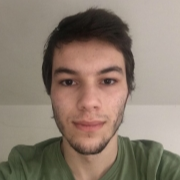
\includegraphics[width=\linewidth]{images/capa/152.png}
            \centering
            \captionsetup{A89458}
        \endminipage\hfill
        \minipage{0.32\textwidth}
            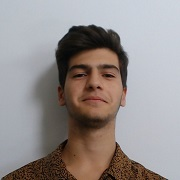
\includegraphics[width=\linewidth]{images/capa/133.jpeg}
            \centering
            \captionsetup{A89585}
        \endminipage\hfill
        \minipage{0.32\textwidth}
            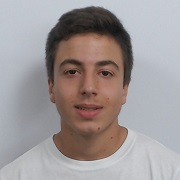
\includegraphics[width=\linewidth]{images/capa/80.jpeg}
            \centering
            \captionsetup{A89597}
        \endminipage
        \end{figure}
    \end{center}
\end{titlepage}

\tableofcontents
\thispagestyle{empty}
\cleardoublepage

\setcounter{page}{1}


%------------------------------------------------------------------------------------------------------%
\section{Captura e análise de Tramas Ethernet}

Assegure-se que a cache do seu browser está vazia. Ative o Wireshark na sua máquina nativa. No seu browser, aceda ao URL http://elearning.uminho.pt. Pare a captura do Wireshark.\\

Obtenha o número de ordem da sequência de bytes capturada (coluna daesquerda na janela do Wireshark) correspondente à mensagem HTTP GETenviada pelo seu computador para o servidor Web, bem como o começo da respectiva mensagem HTTP Response proveniente do servidor.\\ 

No sentido de proceder à análise do tráfego, selecione a trama Ethernet que contém a mensagem HTTP GET. Recorde-se que a mensagem GET do HTTP está no interior de um segmento TCP que é transportado num datagrama IP que, por sua vez, está encapsulado no campo de dados de uma trama Ethernet. Expanda a informação do nível da ligação de dados e observe o conteúdo da trama Ethernet (cabeçalho e dados (payload)).\\

Responda às perguntas seguintes com base no conteúdo da tramaEthernet que contém a mensagem HTTP GET.\\

Sempre que aplicável, deve incluir a impressão dos dados relativa ao pacote capturado (ou parte dele) necessária para fundamentar a resposta à questão colocada. Selecione o mínimo detalhe necessário para responder à pergunta.

\vspace{0.5cm}

\subsection{Pergunta 1}

\textbf{Anote os endereços MAC de origem e de destino da tramacapturada.}

Endereço MAC de origem:  90:32:4b:a8:61:37

Endereço MAC de destino:  00:d0:03:ff:94:00

\begin{figure}[hbt!]
    \centering
    \frame{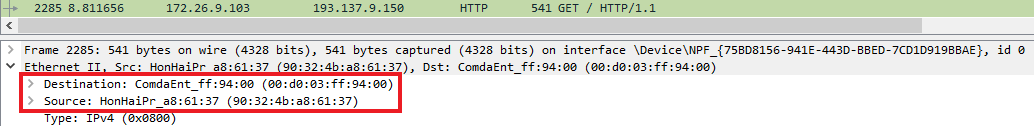
\includegraphics[width=1\textwidth]{images/cap3/pacote_http_get.png}}
    \caption{Trama Ethernet que contém a mensagem HTTP GET}
\end{figure}
\clearpage

\subsection{Pergunta 2}

\textbf{Identifique a que sistemas se referem. Justifique.}

O endereço MAC de origem refere-se ao endereço físico do nosso computador e o de destino refere-se ao endereço físico do router com que se comunicou.

\subsection{Pergunta 3}

\textbf{Qual o valor hexadecimal do campo Type da trama Ethernet? O quesignifica?}

O valor hexadecimal do campo Type, observado na figura 1, tem o valor 0x0800. Significa que o payload da trama contém um datagrama IPv4.

\subsection{Pergunta 4}

\textbf{Quantos bytes são usados desde o início da trama até ao caractere ASCII “G” do método HTTP GET? Calcule e indique, em percentagem, a sobrecarga (overhead) introduzida pela pilha protocolar no envio do HTTP GET.}

O caractere "G" encontra-se no byte 0x37, logo são usados 54 bytes até lá (0x36 = 3*16+6 = 54). Como a trama tem 541 bytes, o overhead é igual a (54 / 541) * 100 = 9.98\%.

\begin{figure}[hbt!]
    \centering
    \frame{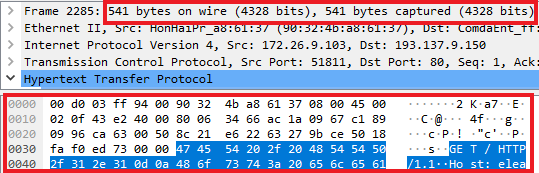
\includegraphics[width=1\textwidth]{images/cap3/bytes_trama.png}}
    \caption{Valor dos bytes da trama}
\end{figure}
\clearpage
\subsection{Pergunta 5}

\textbf{Através de visualização direta ou construindo um filtro específico, verifique se foram detetadas tramas com erros (por verificação do campo FCS (Frame Check Sequence)).}

Como se pode ser na imagem seguinte, após aplicar o filtro "eth.fcs" não detetamos nenhuma trama. Após uma pesquisa, verificámos que, devido aos avanços na tecnologia, é muito incomum as ligações por cabo enviarem packets com erros, pois são muito estáveis.

\begin{figure}[hbt!]
    \centering
    \frame{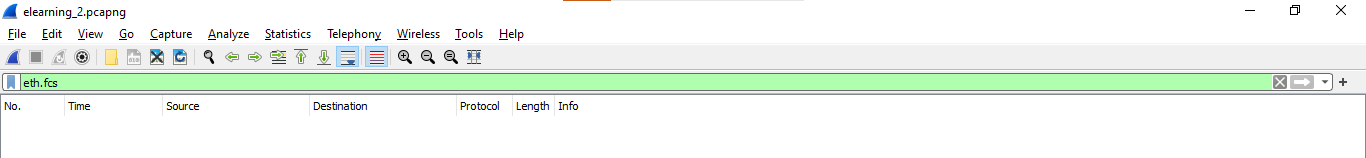
\includegraphics[width=1\textwidth]{images/cap3/filtro_fcs.png}}
    \caption{Filtro para verificação de erros - FCS}
\end{figure}

\vspace{0.5cm}

A seguir responda às seguintes perguntas, baseado no conteúdo da trama Ethernet que contém o primeiro byte da resposta HTTP.

\vspace{0.5cm}

\subsection{Pergunta 6}

\textbf{Qual é o endereço Ethernet da fonte? A que sistema de rede corresponde? Justifique.}

O endereço Ethernet da fonte é 90:77:ee:fa:79:8f e corresponde ao endereço físico do router com que se comunicou, pois este pacote representa a resposta do router ao nosso pedido.

\begin{figure}[hbt!]
    \centering
    \frame{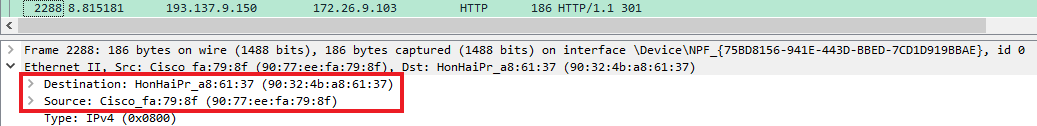
\includegraphics[width=1\textwidth]{images/cap3/pacote_http_reply.png}}
    \caption{Trama Ethernet que contém o primeiro byte da resposta HTTP}
\end{figure}

\subsection{Pergunta 7}

\textbf{Qual é o endereço MAC do destino? A que sistema corresponde?}

Como se pode ver na Figura 3, o endereço MAC do destino é 10:62:e5:87:98:fc e corresponde ao endereço físico da interface ativa do nosso computador.
\clearpage
\subsection{Pergunta 8}

\textbf{Atendendo ao conceito de desencapsulamento protocolar, identifique os vários protocolos contidos na trama recebida.}

A trama recebida contém os seguintes protocolos: Ethernet; IPv4 (Internet Protocol Version 4); TCP (Transmission Control Protocol); HTTP (Hypertext Transfer Protocol).

\begin{figure}[hbt!]
    \centering
    \frame{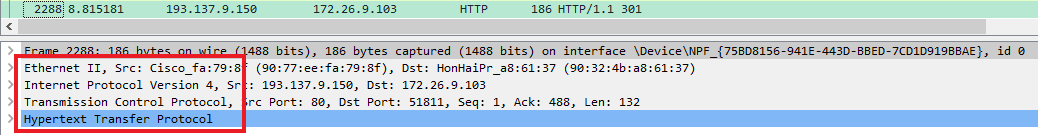
\includegraphics[width=1\textwidth]{images/cap3/protocolos_reply.png}}
    \caption{Protocolos contidos na trama recebida}
\end{figure}

%-----------------------------------------------------------------%

\clearpage
\section{Protocolo ARP}

Nesta secção, pretende-se analisar a operação do protocolo ARP.

Verifique o conteúdo da cache ARP do seu computador.

\vspace{0.5cm}

\subsection{Pergunta 9}

\textbf{Observe o conteúdo da tabela ARP. Diga o que significa cada uma das colunas.}

A primeira coluna representa o endereço IP, a segunda o endereço MAC e a terceira o tipo de endereçamento usado. Cada linha da tabela ARP corresponde a um equipamento que comunicou recentemente com o nosso computador.

\begin{figure}[hbt!]
    \centering
    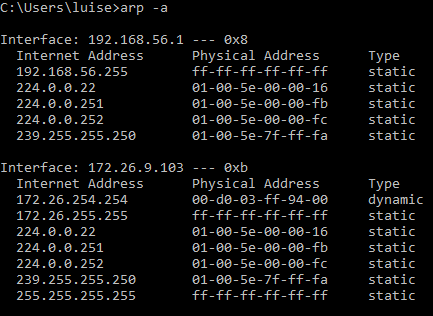
\includegraphics[width=0.7\textwidth]{images/cap4/tabela_ARP.png}
    \caption{Tabela ARP}
\end{figure}

\vspace{0.5cm}

No sentido de observar o envio e recepção de mensagens ARP, é conveniente apagar o conteúdo da cache ARP. Caso contrario, é provável que a associação entre endereços IP e MAC já exista em cache.

Para observar o protocolo ARP em operação, apague novamente a cache ARP e assegure-se que o cache do browser está vazia.
\clearpage
\begin{figure}[hbt!]
    \centering
    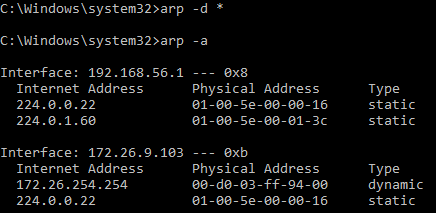
\includegraphics[width=0.7\textwidth]{images/cap4/tabela_ARP_delete.png}
    \caption{Tabela ARP após apagar o conteúdo da cache}
\end{figure}

Inicie a captura de tráfego com o Wireshark, e aceda a http://alunos.uminho.pt. Efectue também um ping para um host da sala de aula que esteja a ser usado por outro grupo. Pare a captura de tráfego e tente localizar o tráfego ARP. Se necessário, limite os protocolos visíveis apenas a protocolos abaixo do nível IP. Para tal, seleccione Analyze->Enabled Protocols e remova a selecção da opção IPv4 e IPv6.

Responda às seguintes perguntas:

\subsection{Pergunta 10}

\textbf{Qual é o valor hexadecimal dos endereços origem e destino na trama Ethernet que contém a mensagem com o pedido ARP (ARP Request)? Como interpreta e justifica o endereço destino usado?}

O endereço de origem na trama Ethernet é igual a 90:32:4b:a8:61:37 e o de destino ff:ff:ff:ff:ff:ff.

O valor do endereço de destino deve-se ao facto de não se conhecer o endereço MAC associado ao endereço IP de destino. Assim, o computador envia um pacote para todos os dispositivos ligados à rede e aquele que tiver o endereço IP de destino (172.26.254.254) responderá, podendo, assim, conhecer-se o seu endereço MAC.

\begin{figure}[hbt!]
    \centering
    \frame{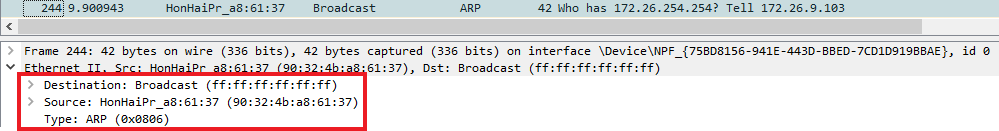
\includegraphics[width=1\textwidth]{images/cap4/ARP_request_ethernet.png}}
    \caption{Pacote ARP Request - Ethernet}
\end{figure}

\subsection{Pergunta 11}

\textbf{Qual o valor hexadecimal do campo tipo da trama Ethernet? O que indica?}

Como se pode verificar na Figura 7, o campo tipo da trama Ethernet tem o valor 0x0806, correspondente ao ARP.

Este valor indica-nos o protocolo usado no tipo de dados da trama.

\subsection{Pergunta 12}

\textbf{Como pode confirmar que se trata efetivamente de um pedido ARP? Identifique que tipo de endereços estão contidos na mensagem ARP? Que conclui?}

Trata-se de um pedido ARP, pois o opcode da camada ARP do pacote é igual a 1 (request) e o endereço MAC de destino é igual a 00:00:00:00:00:00.

Na mensagem ARP estão contidos os endereços MAC e IP, de origem e de destino. Conclui-se que este protocolo serve para associar um endereço MAC a um endereço IP de uma interface ativa.

\begin{figure}[hbt!]
    \centering
    \frame{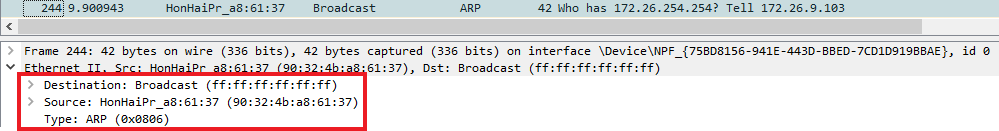
\includegraphics[width=1\textwidth]{images/cap4/ARP_request_ethernet.png}}
    \caption{Pacote ARP Request - ARP}
\end{figure}

\subsection{Pergunta 13}

\textbf{Explicite que tipo de pedido ou pergunta é feita pelo host de origem?}

O host de origem pergunta quem tem o IP 172.26.254.254 e indica que o seu IP é 172.26.9.103. Assim, o host consegue descobrir o endereço MAC associado ao IP 172.26.254.254, pois este envia o pedido a todos os dispositivos ligados à rede.
\clearpage
\subsection{Pergunta 14}

Localize a mensagem ARP que é a resposta ao pedido ARP efetuado.

\vspace{0.5cm}

\textbf{A - Qual o valor do campo ARP opcode? O que especifica?}

O valor do campo opcode é 2. Isto indica que o pacote ARP é uma resposta a um ARP Request.

\begin{figure}[hbt!]
    \centering
    \frame{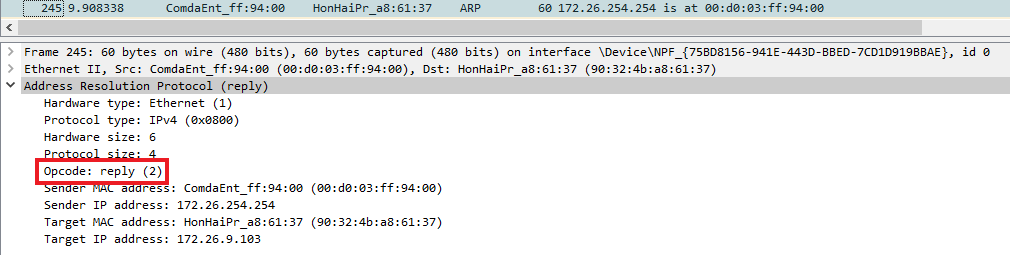
\includegraphics[width=1\textwidth]{images/cap4/ARP_reply.png}}
    \caption{Campo opcode do pacote ARP Reply}
\end{figure}

\vspace{0.5cm}

\textbf{B - Em que posição da mensagem ARP está a resposta ao pedido ARP?}

A resposta ao pedido ARP está entre as posições 0x16 e 0x1b, pois é onde se encontra o endereço MAC de origem.

\begin{figure}[hbt!]
    \centering
    \frame{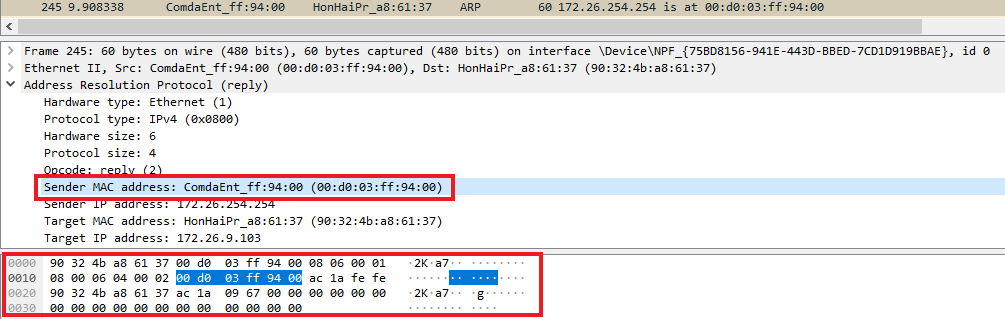
\includegraphics[width=1\textwidth]{images/cap4/ARP_reply_posicao.png}}
    \caption{Posição da resposta na mensagem ARP}
\end{figure}



%-----------------------------------------------------------------%

\clearpage
\section{ARP Gratuito}

Arranque o Wireshark na sua máquina nativa e inicie a captura de dados. Desligue e volte a ligar a sua ligação à rede local, ou force o pedido de atribuição de um novo endereço IP à interface em uso. Pare a captura de tráfego. Utilize o filtro de visualização ARP para facilitar a identificação dos pacotes respetivos.

\vspace{0.5cm}

\subsection{Pergunta 15}

\textbf{Identifique um pacote de pedido ARP gratuito originado pelo seu sistema. Analise o conteúdo de um pedido ARP gratuito e identifique em que se distingue dos restantes pedidos ARP. Registe a trama Ethernet correspondente. Qual o resultado esperado face ao pedido ARP gratuito enviado?}

O pedido ARP gratuito selecionado distingue-se dos outros pedidos ARP por ter o mesmo IP de origem e de destino. Desta forma, o computador pretende saber se existe outro equipamento na rede com o mesmo IP, pois, caso exista, este irá responder ao pedido ARP. Neste caso em estudo, o computador não recebeu resposta ao pedido, logo não há conflito de IP's na rede.

\begin{figure}[hbt!]
    \centering
    \frame{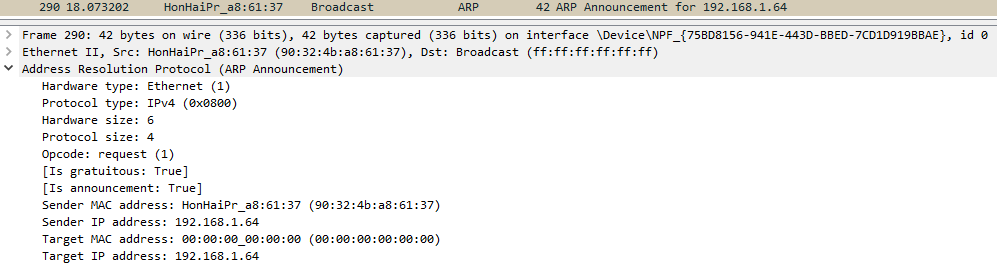
\includegraphics[width=1\textwidth]{images/cap5/ARP_announcement.png}}
    \caption{ARP Announcement}
\end{figure}




%-----------------------------------------------------------------%

\clearpage
\section{Domínios de colisão}

Ative o emulador CORE e carregue a topologia de rede com a solução de subnetting que construiu no âmbito do TP2. Substitua o switch do departamentos B por um hub (repetidor).

\begin{figure}[hbt!]
    \centering
    \frame{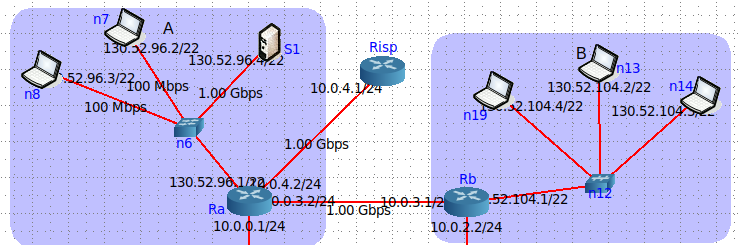
\includegraphics[width=1\textwidth]{images/cap6/CORE.png}}
    \caption{Topologia CORE em estudo}
\end{figure}

\subsection{Pergunta 16}

\textbf{Através da opção tcpdump verifique e compare como flui o tráfego nas diversas interfaces dos vários dispositivos no departamento A (LAN comutada) e no departamento B (LAN partilhada) quando gera tráfego intra-departamento (por exemplo, através do comando ping). Que conclui?}

\textbf{Comente os resultados obtidos quanto à utilização de hubs e switches no contexto de controlar ou dividir domínios de colisão. Documente as suas observações e conclusões com base no tráfego observado/capturado.}

Inicialmente estudamos o comportamento no departamento A (LAN comutada).

Neste caso, executamos o comando ping de n7 para n8. Assim, o laptop n7 começa por enviar uma pacote de request para o laptop n8. Quando o pacote chega ao switch, este envia um ARP broadcast para todos os equipamentos ligados a ele, de forma a descobrir a que porta está ligado o n8. Depois, o switch guarda essa informação na sua tabela de endereçamento. A partir desse momento, quando n7 comunica com n8 (e vice-versa) o switch simplesmente reencaminha o pacote para o destino, através da informação guardada na tabela.

Na imagem seguinte podemos confirmar que o tráfego no servidor S1 corresponde apenas ao ARP broadcast, enquanto que nos equipamentos n7 e n8 encontramos o pacote ARP brodcast e a sua resposta e os pacotes referentes ao comando ping.

\begin{figure}[hbt!]
    \centering
    \frame{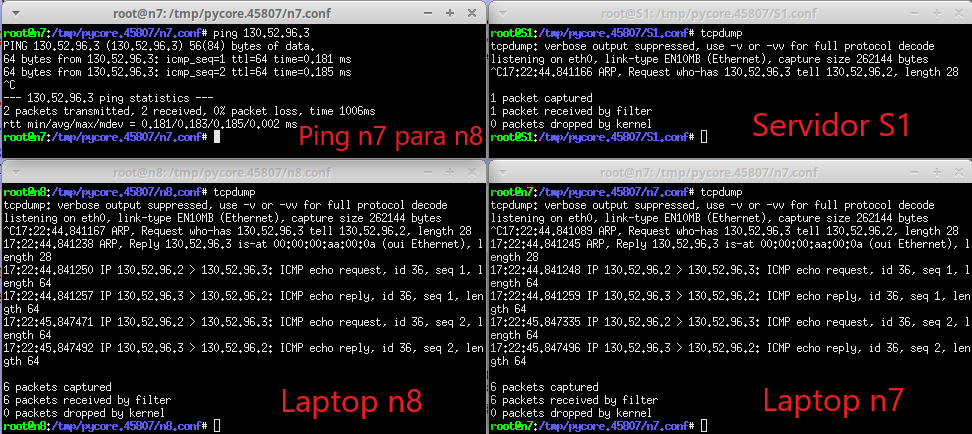
\includegraphics[width=1\textwidth]{images/cap6/trafego_switch.png}}
    \caption{Tráfego no departamento A (LAN comutada)}
\end{figure}
\clearpage

Depois de termos estudado o comportamento de um switch, estudamos o comportamento do departamento B (LAN partilhada).

Neste caso, executamos o compando ping de n13 para n14. O procedimento e o tráfego nos laptops relacionados ao comando ping são iguais aos referidos no exemplo anterior. A única diferença está no tráfego do laptop n19 (comparando ao servidor S1 do exemplo anterior). Isto deve-se ao facto de o hub distribuir os pacotes para todos os equipamentos ligados a si, mesmo depois de conhecer a localização de n13 e n14.

Na imagem seguinte verificamos que o tráfego é igual nos três equipamentos ligados ao hub.

\begin{figure}[hbt!]
    \centering
    \frame{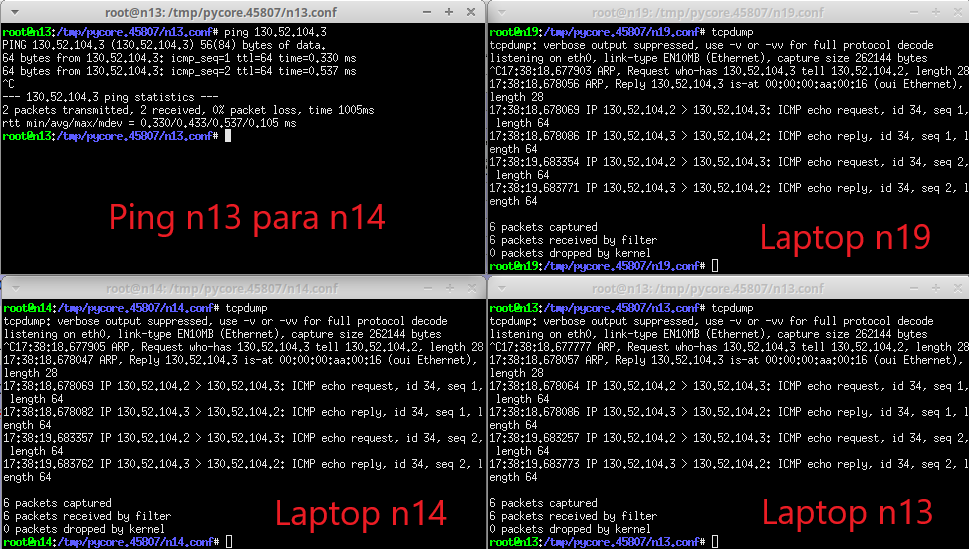
\includegraphics[width=1\textwidth]{images/cap6/trafego_hub.png}}
    \caption{Tráfego no departamento B (LAN partilhada)}
\end{figure}
\clearpage

\section{Conclusão}

Neste trabalho prático, começamos por analisar o tráfego Ethernet e perceber o seu comportamento através do Wireshark. Também estudamos o protocolo ARP, percebendo melhor como funciona o endereçamento numa sub-rede.

Para finalisar, verificamos a diferença entre a utilização de um hub ou de um switch para efetuar a interligação entre dispositivos numa sub-rede.

\end{document}
